\documentclass{sigchi}

% Use this command to override the default ACM copyright statement
% (e.g. for preprints).  Consult the conference website for the
% camera-ready copyright statement.


%% EXAMPLE BEGIN -- HOW TO OVERRIDE THE DEFAULT COPYRIGHT STRIP -- (July 22, 2013 - Paul Baumann)
% \toappear{Permission to make digital or hard copies of all or part of this work for personal or classroom use is      granted without fee provided that copies are not made or distributed for profit or commercial advantage and that copies bear this notice and the full citation on the first page. Copyrights for components of this work owned by others than ACM must be honored. Abstracting with credit is permitted. To copy otherwise, or republish, to post on servers or to redistribute to lists, requires prior specific permission and/or a fee. Request permissions from permissions@acm.org. \\
% {\emph{CHI'14}}, April 26--May 1, 2014, Toronto, Canada. \\
% Copyright \copyright~2014 ACM ISBN/14/04...\$15.00. \\
% DOI string from ACM form confirmation}
%% EXAMPLE END -- HOW TO OVERRIDE THE DEFAULT COPYRIGHT STRIP -- (July 22, 2013 - Paul Baumann)


% Arabic page numbers for submission.  Remove this line to eliminate
% page numbers for the camera ready copy 

%\pagenumbering{arabic}

% Load basic packages
\usepackage{balance}  % to better equalize the last page
% \usepackage{graphics} % for EPS, load graphicx instead 
%\usepackage[T1]{fontenc}
\usepackage{txfonts}
\usepackage{times}    % comment if you want LaTeX's default font
\usepackage[pdftex]{hyperref}
% \usepackage{url}      % llt: nicely formatted URLs
\usepackage{color}
\usepackage{textcomp}
\usepackage{booktabs}
\usepackage{ccicons}
\usepackage{todonotes}
\usepackage{xltabular}
\usepackage{graphicx}
\usepackage{multicol}
% \usepackage{subfig}

% llt: Define a global style for URLs, rather that the default one
\makeatletter
\def\url@leostyle{%
  \@ifundefined{selectfont}{\def\UrlFont{\sf}}{\def\UrlFont{\small\bf\ttfamily}}}
\makeatother
\urlstyle{leo}

% To make various LaTeX processors do the right thing with page size.
\def\pprw{8.5in}
\def\pprh{11in}
\special{papersize=\pprw,\pprh}
\setlength{\paperwidth}{\pprw}
\setlength{\paperheight}{\pprh}
\setlength{\pdfpagewidth}{\pprw}
\setlength{\pdfpageheight}{\pprh}

% Make sure hyperref comes last of your loaded packages, to give it a
% fighting chance of not being over-written, since its job is to
% redefine many LaTeX commands.
\definecolor{linkColor}{RGB}{6,125,233}
\hypersetup{%
  pdftitle={CSCM79: Hardware \& Devices Coursework Report - The Every Dice},
  pdfauthor={LaTeX},
  pdfkeywords={dice, hardware, devices, coursework, report, cscm79},
  bookmarksnumbered,
  pdfstartview={FitH},
  colorlinks,
  citecolor=black,
  filecolor=black,
  linkcolor=black,
  urlcolor=linkColor,
  breaklinks=true,
}

% create a shortcut to typeset table headings
% \newcommand\tabhead[1]{\small\textbf{#1}}

% End of preamble. Here it comes the document.
\begin{document}

\title{CSCM79: Hardware \& Devices Coursework Report \\- The Every Dice}

\numberofauthors{4}
\author{%
  \alignauthor{Jamie Bragg\\
    \affaddr{2137481}}\\
  \alignauthor{Sean Coaker\\
    \affaddr{986529}}\\
  \alignauthor{Dylan Parry\\
    \affaddr{961883}}\\
  \alignauthor{Ryan Lucas\\
    \affaddr{951998}}\\
}

\maketitle

\begin{abstract}

 This document reports on our hardware device. It explains the motivation behind the device, defines the requirements, details the implementation and evaluates the device along with a discussion of the concepts utilised.

\end{abstract}

\section{Introduction}

Anxiety has been studied as a problem occurring within classrooms where certain teaching practices put pressure on students and can cause excess stress. This anxiety, caused primarily by the tactic of calling on a specific student to answer questions, has also been seen as a link to general social anxiety and lower grades.  

Active learning is a method of teaching where the students are actively involved in the learning process through discussion, debate, and tasks that help the student develop their understanding of a topic as they work through it. 

However, the problems become apparent when you see that active learning also uses techniques which increase anxiety in the classroom. These techniques, whilst beneficial to those without anxiety, can be seen as stress inducing to students suffering with anxiety, rendering it less useful. For active learning to be effective, there must be ways to adapt it to students who suffer from anxiety. 

To address the problem of anxiety in the classroom, this report wSill investigate the viability of using technology in an active learning environment, with the goal of reducing anxiety whilst retaining the effectiveness of active learning. By doing so, this report should be able to develop a prototype of a product that could achieve this task. 

\section{Literature Review}

Active learning is defined as “a method of learning in which students are actively or experientially involved in the learning process.” \cite{bonwell_eison_1991}. It is seen as a beneficial teaching method in which students are actively involved in the learning process. This can be accomplished through tools such as class discussions and debates where the students are encouraged to talk to one another or the teacher to generate a greater understanding of the topic. The benefits of active learning are apparent, with active learning reducing the failure rates of students in classes where it is used \cite{freeman_eddy_mcdonough_smith_okoroafor_jordt_wenderoth_2014}.  

Benjamin England et al. studied anxiety in the classroom. They conducted surveys and interviews with students about which active learning practices caused them to feel anxious. The classroom practices that lead to the most anxiety were different ways of questioning. Cold calling, a practice were the teacher selects a specific student to answer, was the most anxiety inducing while volunteer questioning was the second most anxiety inducing. The reasons that the students gave for feeling anxiety were a mixture of communication apprehension, social anxiety and test anxiety. This demonstrates a problem in the classroom as the authors found that anxiety could have potential impacts on student grades as those who felt stronger anxiety tended to have lower grades \cite{england_brigati_schussler_2017}.

Active learning techniques have been shown to be beneficial to students despite the concerns about anxiety. Shams Huda et al conducted a study into the benefits of active learning strategies. They found that active learning strategies increased student engagement and participation. Students were also found to have learnt more through active learning strategies. They also found that two thirds of the students also felt that active learning techniques were beneficial to them, this is backed up with an increase in student grades. This paper demonstrates that active learning is an overall positive learning environment. The issue of anxiety shown by Benjamin is the only hurdle found that could lead to students having a bad experience and lower grades. We have designed The Every Dice with the goal of combatting the problem of anxiety when answering questions in the classroom \cite{ul_huda_ali_nanji_cassum_2016}.

\section{Requirements and Specifications}

This section includes a brief description for the requirements and specifications of the project. The following table, table \ref{tbl:func_reqs_table}, lists the requirements of the Every Dice project along with accompanying specifications that needed to be met to allow each requirement to be attained successfully.

\onecolumn
\vspace{2em}
\small
\begin{xltabular}[H]{\textwidth}{c | X | X}
    \caption[Requirements and Specifications]{A table of requirements with relative specifications that need to be met to reach the requirement.}\\

    \toprule

    Code & User Requirement & Specification\\

    \midrule
    \endfirsthead

    \toprule

    Code & User Requirement & Specification\\

    \midrule
    \endhead

    \hline
    \multicolumn{3}{|r|}{{Continued on next page}}\\
    \hline
    \endfoot

    \bottomrule
    \endlastfoot

    REQ1

    &

    The Every Dice should allow the user to answer questions in an attempt to reduce anxiety in classrooms that practise active learning.

    &

    The Android application should allow a user to list options for answers and select the correct answer. This has been implemented with a recycler view that allows the user to add and remove items to and from the list.\\

    \cmidrule{3-3}

    &

    &

    When a user sets down the Every Dice, the side facing up, determined by the contained spacial phidget, will become the chosen answer. At this point, the user can tap the 'check answer' button in the application and communication between the Every Dice, and the Android application should ensure that the user is notified whether their answer is incorrect or correct with a display on the screen facing upwards and an audio tone.\\

    \midrule

    REQ2

    &

    The Every Dice should permit the size of the dice to be greater than 6 sides. Allowing for the Every Dice to be used in games that require dices with varying shapes of dice.

    &

    The Android application should include a state machine feature that ensures that the Every Dice is notified when the number of items listed in the application are greater than 6 sides, with the Every Dice having virtually more than 6 sides.\\

    \cmidrule{3-3}

    &

    &

    In this instance, instead of displaying each item on each side as the application does when 6 items are selected, the application should animate each screen, with a shuffle through each of the items listed in the application.\\

    \cmidrule{3-3}

    &

    &

    The application should make a pseudo-random choice of one of the listed items. Once an external spatial phidget has been shaken, the selected pseudo-random item is displayed to the side facing upwards as the chosen side. The side facing upwards will again be determined by the internal spatial phidget.\\

    \midrule

    REQ3

    &

    The Every Dice should facilitate an auto-roll feature, for entertainment purposes and for the purpose of a user being able to auto-roll a random answer when they are unsure of a question within a classroom setting.

    &

    With a shake of the mobile phone device the application will send a prompt to the Every Dice to auto-roll. The Every Dice should use the servo motors contained within the dice housing to open each side to roll the dice over a random number of times.\\

    \midrule

    REQ4

    &

    The Every Dice should include ambient media and be able to stand out in the foreground and be able to blend into the background.

    &

    With the use of contexts in the Android application lifecycle, we can identify when the user is no longer using the Every Dice. When this occurs, the dice will play a sleep audio tone before turning off all screens and disabling the phidget hardware. When the application becomes the main focus of the mobile device again, the Every Dice plays a start audio tone and the screens are displayed once again after all phidgets have been restarted.\\

    \midrule

    REQ5

    &

    Include interactive surfaces to represent an everyday or intuitive physical object as a tangible computing device. 

    &

    Create a cube device that include screens on all sides. This represents interactive surfaces as a dice.\\

 \midrule

    REQ6

    &

   Include interactions between Bits and Atoms that allow for changes in the digital world to affect the device physically. Also changes in the physical world must affect the digital world. 

    &

   To allow for physical movement to affect the digital world, the user should be able to shake their phone to activate the dice roll function. For the digital world affecting the physical device, the app should be able to activate the autoroll feature, physically moving the dice from the digital app.\\

\end{xltabular}
\label{tbl:func_reqs_table}


\twocolumn
\section{Implementation}

The completed first prototype is a package that involves a wooden housing containing all the necessary phidget hardware to implement the Every Dice system. As well as the hardware included in the dice housing, an external spatial phidget is utilised to identify when the dice has been rolled. This decision was made to avoid the prototype itself needing to be rolled, which would have increased the likelihood of causing damage to the dice. An overview of the cutouts to each side of the dice can be seen in figure \ref{fig:dice_cutouts}.

  % [H] means put the figure HERE, directly when you input this code.
\begin{figure}[ht!]
	\centering

% We set the width of the figure based on the width of one line of text on the page. 
% The value can be tuned to any value in [0.0, 1.0] to scale the image while maintaining its aspect ratio.

	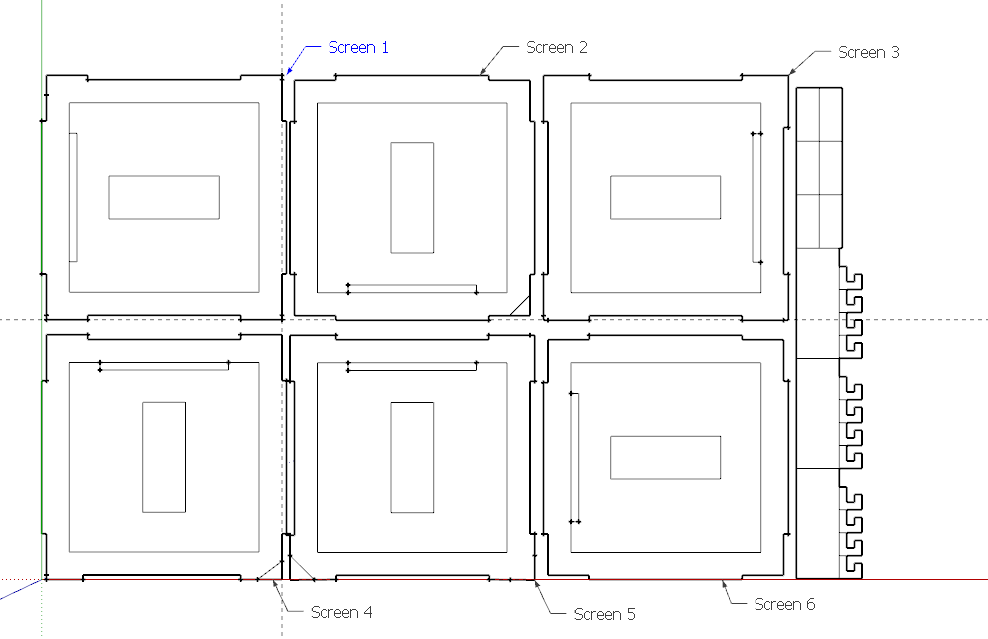
\includegraphics[width=1.0\linewidth]{./figures/cutouts.png}
	
% Caption is defined with a short and long version. The short version is shown in the 
% List of Figures section, and the long version is used directly with the figure. 		
	\caption[Every Dice Side Cutouts]{A model of the cutouts of each side that needed to be created to form the Every Dice.}
	
% For figures label should be defined after the caption to ensure proper figure numbering.
	\label{fig:dice_cutouts}
	
\end{figure}

As stated previously, the necessary hardware to implement the features required for the project were housed within the dice's wooden casing. Each side acts as a door which has two uses, provide access to the hardware of the device to allow for easy adjustments during prototyping, and to allow for the auto-roll feature of the device to be implemented. Due to resource constraints, we could only implement 3 doors for the auto-roll feature, but they provide a proof-of-concept of how we envisioned this feature working. Each of the 3 working doors are connected to servo-motors which allow them to be opened. The theory behind this is that the opening motion would press the door against the surface it is sat on, causing the dice to flip over to another side. An example of the built prototype containing its hardware contents can be viewed in figure \ref{fig:dice_hardware}.

  % [H] means put the figure HERE, directly when you input this code.
\begin{figure}[ht!]
	\centering

% We set the width of the figure based on the width of one line of text on the page. 
% The value can be tuned to any value in [0.0, 1.0] to scale the image while maintaining its aspect ratio.

	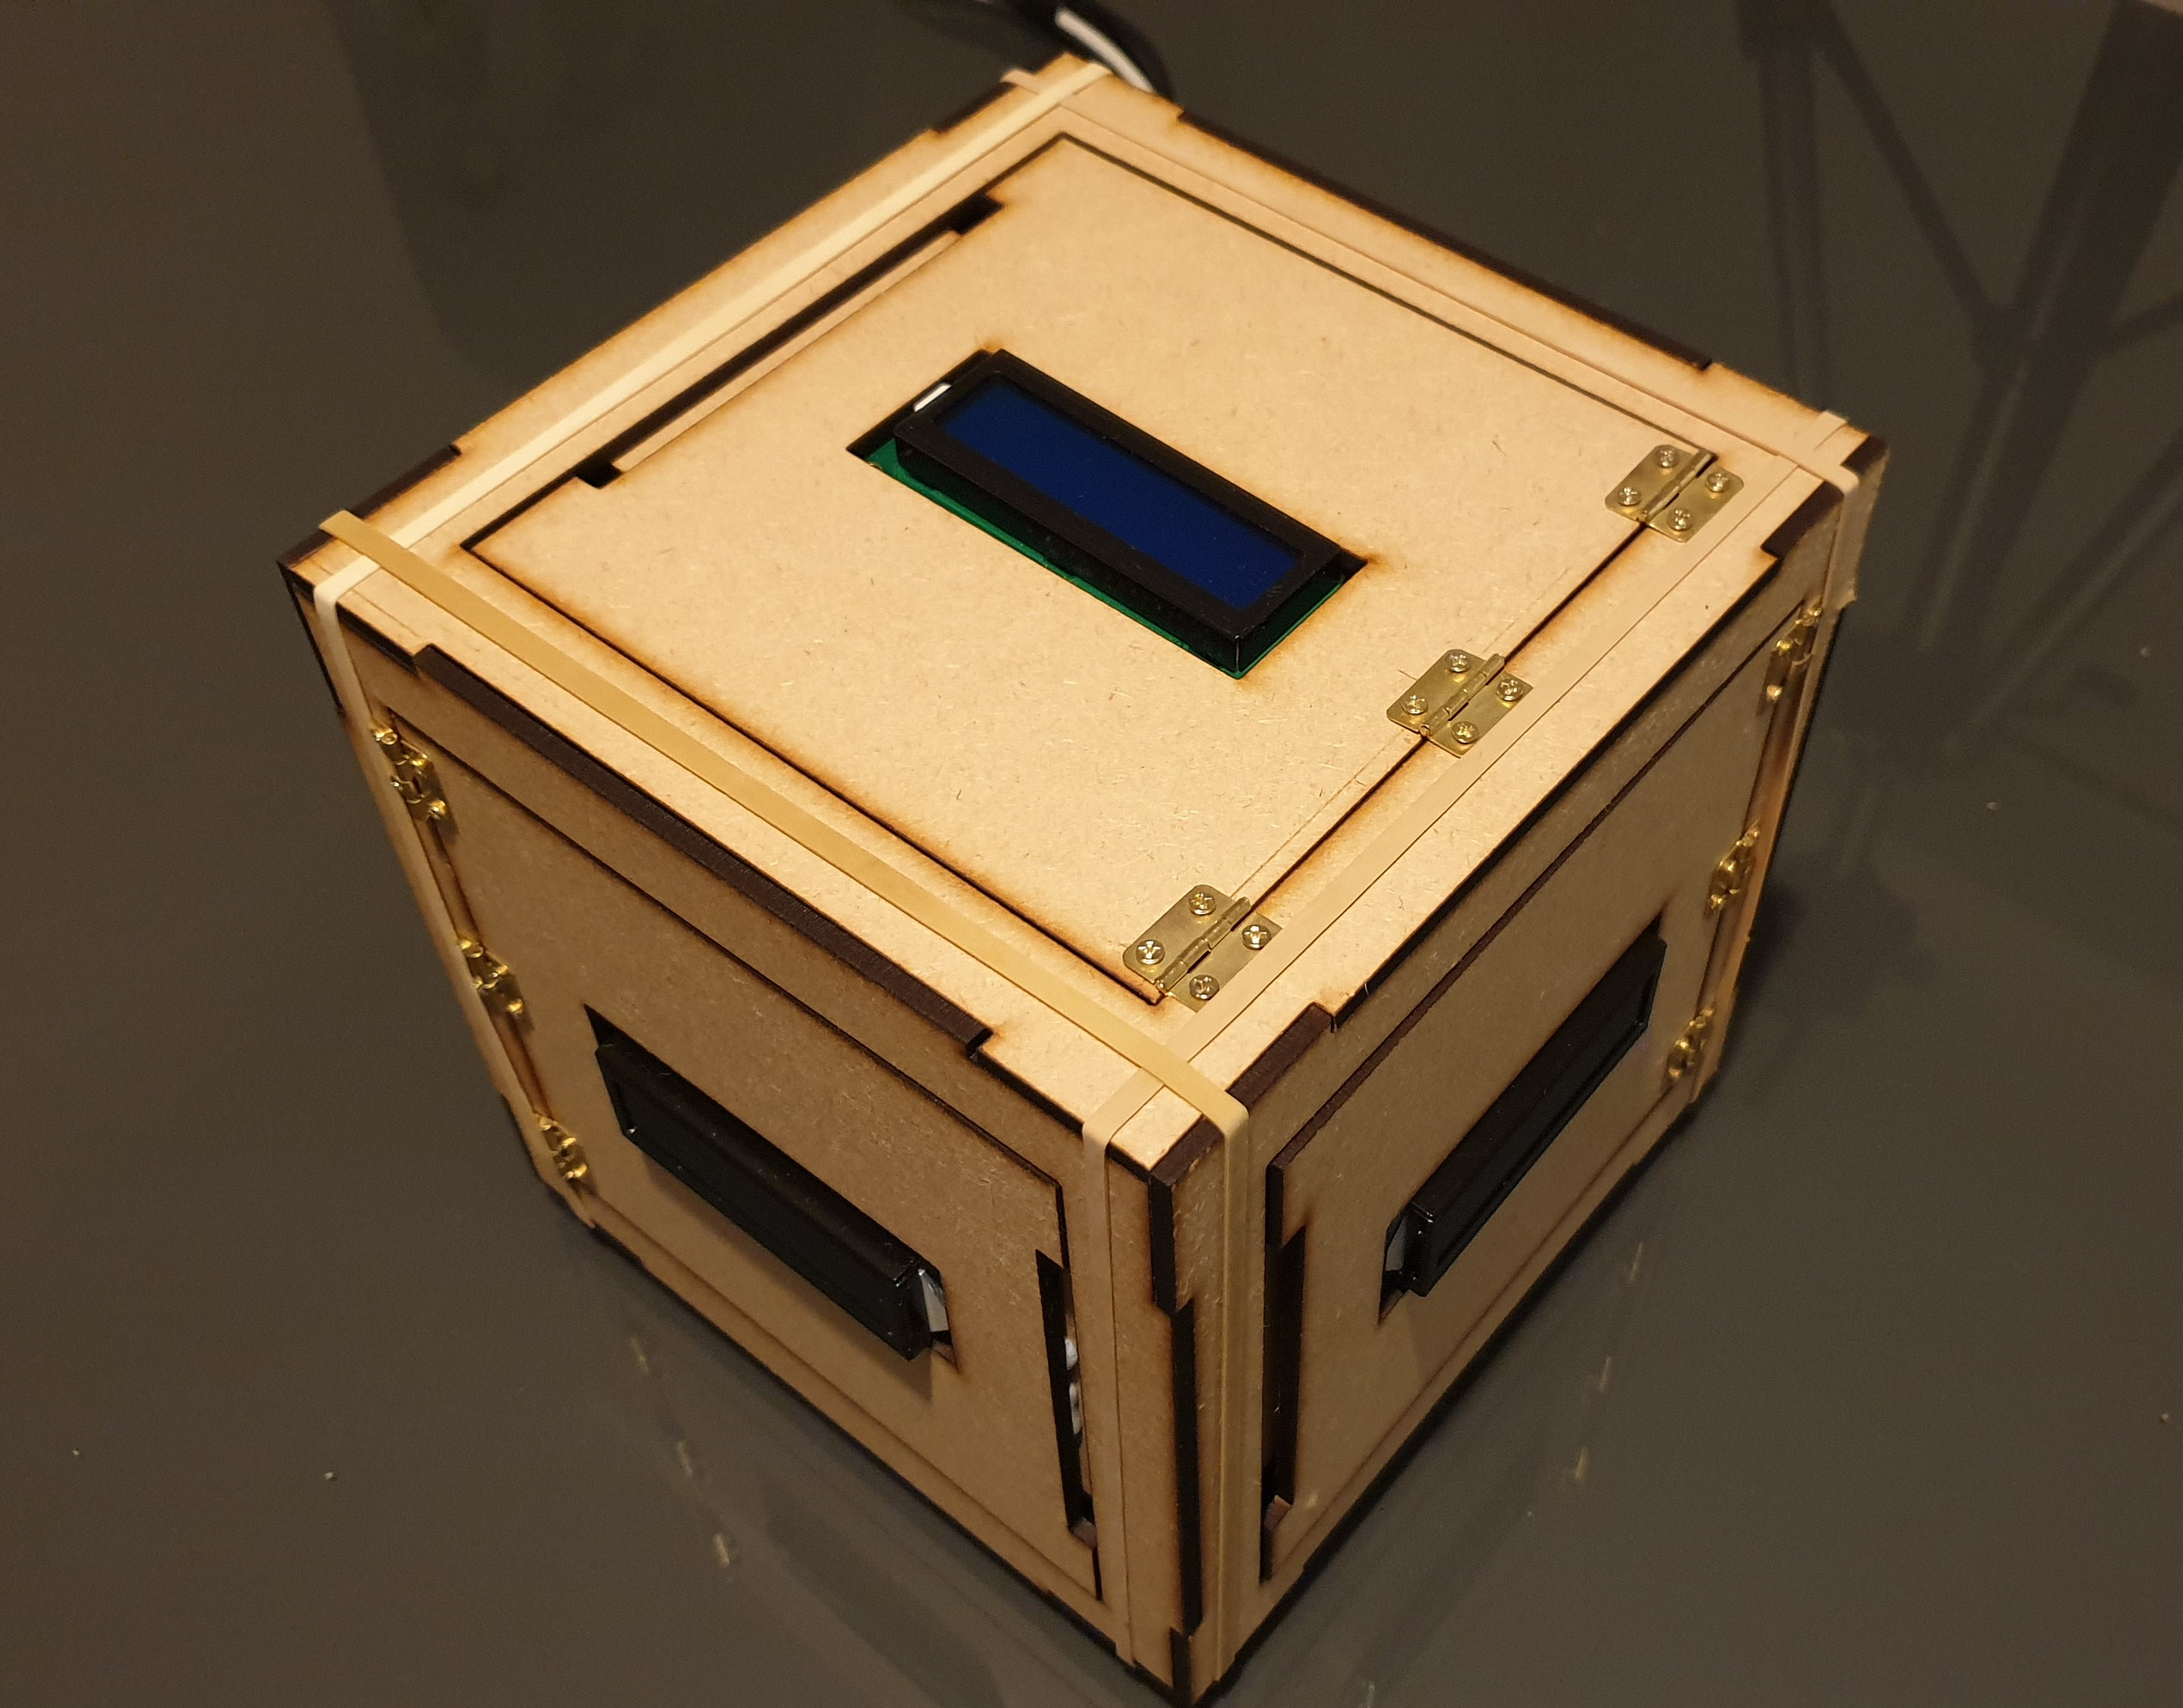
\includegraphics[width=0.8\linewidth]{./figures/hardware.jpg}
	
% Caption is defined with a short and long version. The short version is shown in the 
% List of Figures section, and the long version is used directly with the figure. 		
	\caption[The Built Every Dice]{An image of the built Every Dice prototype.}
	
% For figures label should be defined after the caption to ensure proper figure numbering.
	\label{fig:dice_hardware}
	
\end{figure}

Another important piece of hardware that is included within the casing of the prototype is the internal spatial phidget. This phidget is in constant communication with the application, so it understands which side of the device is currently facing upwards. This is important in allowing us to develop the check answer feature for classroom settings, as well as the feature that allows the dice to be more than 6 sides virtually. A final list of hardware included within this project can be viewed below.

\begin{itemize}
    \item \textbf{2x Spatial Phidget} - One internally to identify which side of the dice is facing upwards, and one externally to help simulate the rolling of the dice.
    \item \textbf{6x LCD Screens} - A screen for each side of the dice.
    \item \textbf{3x LCD Screen Controllers} - Each one used to handle the transferring of data from the application to 2 LCD screens.
    \item \textbf{3x Servo Motors} - Each one used to open the doors of the dice to facilitate the auto-roll feature.
    \item \textbf{1x Buzzer} - Used to play tones when the incorrect/correct answer is detected, or when the dice is being transferred between sleep and awake states.
  \end{itemize}

On the Android application side, we began by developing a MainActivity file that would handle the context change detection of the application, handle the events of each phidget device we have detected, as well as handling the creation of the MainFragment which displays the user interface. The MainActivity class begins by initialising the dice to be in inactive mode using the enum state 'INACTIVE'. Each side of the dice is then set with a generic name. A sensor manager is then created to allow us to handle the detection of the phone shaking and call the auto-roll feature. The communication between each phidget device is then opened ready for communication throughout the application's lifecycle. 

Once the main features of our system are initialised, we include code to handle the context change events. This code ultimately allows the device to turn on and off depending on if the application is in focus on the connected mobile device or not. Alongside this, the options menu for the application is configured to include two buttons. The first of those buttons is the check answer button, one that allows the user of the application to check if the side of the dice that is facing upwards is the same item that they have selected to be the correct answer. The other button is a list reset function which allows the user to quickly clear all items they have selected to be displayed on the dice.

The most important development of code is included within the latter stages of the MainActivity class, which handles the detection of which side of the dice is facing upwards. This is achieved by taking measurements for the x angle and y angle of the accelerometer, before comparing those values to pre-determined threshold values to interpret which side of the dice is facing upwards. Determining the side of the dice that is facing upwards was imperative to being able to implement the check answer feature and determine which side of the dice the user had chosen as their answer, as well as being able to implement the roll feature which floats the pseudo-random item from the user's list to the side facing upwards whenever the dice has more than 6 items chosen and the external spatial phidget is shaken. Other code is also included here to detect changes in acceleration from the external spatial phidget, before comparing those values to a threshold value to determine when the external spatial phidget is being shaken. At this stage, we can perform the roll feature for the dice when more than 6 items have been entered by the user. 

Finally, the work within the MainActivity class is completed with the inclusion of code to handle the background-foreground feature of the Every Dice. Effectively, we have included code that allows audio tones to be played when the dice is going from a sleep state to an awake state, or from an awake state to a sleep state. As well as this, we have included code that allows the LCD screens of the dice to also be switched on and off depending on if the dice is supposed to be sleeping or not.

Aside from the MainActivity class, we have developed two other classes to handle the controlling of the user interface fragment as well as the recycler view within the main fragment, which is used to display the user's selected items through the mobile device. The MainFragment class allows the user to tap on the 'Add Choices...' button and list comma-separated strings that act as their list of options. This list of strings is the data source for both the recycler view and the options to be listed on the dice. Each item in the list is displayed as a card view that includes a delete button for each item to allow the item to be removed from the list. An item in the list can also be selected as the 'correct answer', which is then used as comparison against the item on the side facing upwards on the dice when the check answer button is tapped. The clear button in the options menu also allows the user quickly delete all items from their list, as stated earlier in this section. Within all this code, communication is regularly occurring between the MainActivity and MainFragment to update the state of the dice depending on the number of items selected by the user. An example of the Android application's user interface can be seen in figure \ref{fig:ui}.

% [H] means put the figure HERE, directly when you input this code.
\begin{figure}[ht!]
	\centering

% We set the width of the figure based on the width of one line of text on the page. 
% The value can be tuned to any value in [0.0, 1.0] to scale the image while maintaining its aspect ratio.

	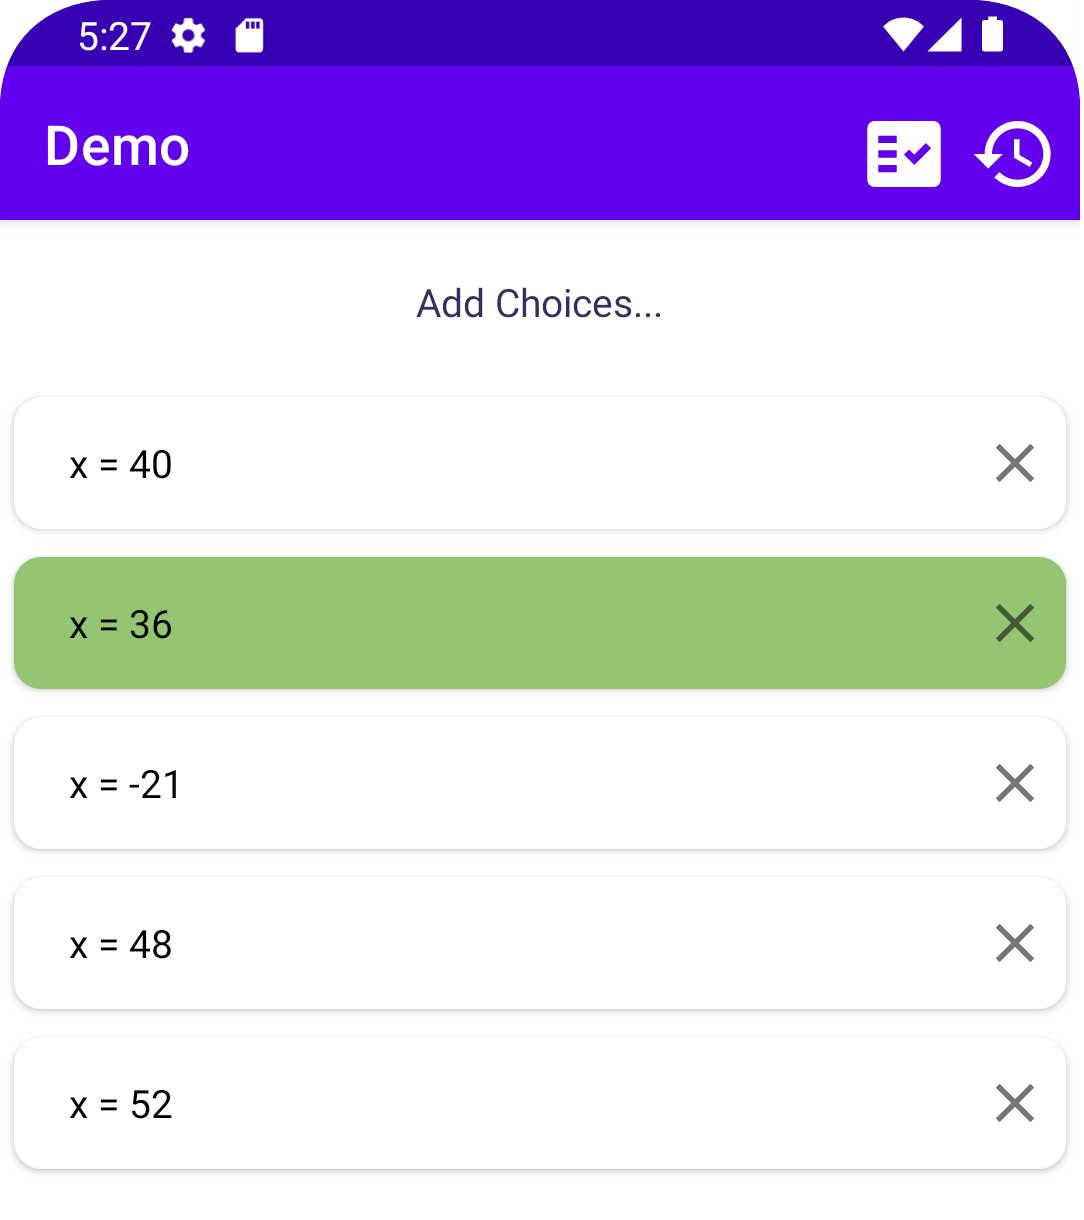
\includegraphics[width=0.8\linewidth]{./figures/ui.png}
	
% Caption is defined with a short and long version. The short version is shown in the 
% List of Figures section, and the long version is used directly with the figure. 		
	\caption[The UI of the Android Application]{An image of the finalised user interface of the Android application.}
	
% For figures label should be defined after the caption to ensure proper figure numbering.
	\label{fig:ui}
	
\end{figure}


\section{Evaluation}

 The EveryDice is a successful project as it was able to meet, or partially meet, all of the requirements. The device allows the user to answer questions using the dice, therefore REQ1 is partially met. We would need to test this wish real users in a school setting before fully meeting REQ1. REQ2 is met as the app allows for the input of more than 6 options. Once rolled, the dice picks an option to be displayed on the top of the screen. The app includes an option for autoroll, when this is activated the dice servos move the dice automatically. Due to the size of the dice, only 3 servos were included in the prototype; a complete version will include 6 servos, one for each side. This results in the partial completion of REQ3. REQ4 requires ambient media. This is included as the dice makes an alert sound and the screens turn on when it is time to be used. The screens turn off when the app is not being used or when the app loses focus. We successfully placed our hardware inside a cube chassis, representing our interactive surface as a dice, this allows the device to meet REQ5. Finally, REQ6 is met as we included a spatial phidget that takes physical movement as an input which activates the roll function and returns a digital output. The app also controls the autoroll feature. These two features allow bits to interact with atoms and atoms to interact with bits. 

While the device is successful, the prototype can be developed further. Firstly, the wires restrict the movement of the dice; wireless technology can resolve this. Also, the device is a lot larger than a regular dice, making the dice smaller would make it resemble a regular dice better, and convey the affordances better. It can also include LEDs that light up to convey correct or incorrect, instead of relying on the user to read the words on the screen. 

\section{Discussion}

The developed prototype of the Every Dice is a tangible user interface. This is because the device can be held physically in the users’ hand and the interaction involves rolling the device as you would a regular dice. This interaction matches the affordances of the tangible dice that the device is imitating. The device lacks persistent tangibles, when the dice is off so are the screens so the user cannot see what is on each face of the dice, they’ll just see a cube. Having said this, as the dice is still designed as a normal dice, nothing stops the user from being able to add labels to each side and still use the EveryDice as a dice even when it is turned off. 

Ambient media refers to devices that blend into the background and is unnoticed by the user. The EveryDice makes a beeping sound when the app is opened alerting the students that the dice is ready to be used. This is how the device comes to the foreground. When the app is closed or loses focus, the screens turn off; this is how the device blends into the background. 

Bits and Atoms refers to the interactions between the physical and digital worlds; the EveryDice has multiple interactions between bits and atoms. The user can physically shake their phone, this manifests in the digital world as the dice’s roll function is triggered. Also, the app can activate servos on the dice to roll it automatically, this is an example of how digital input affects physical output. 

The 1st interaction loop happens when the user picks up the dice and moves it in their hands to see the different faces. The 2nd loop occurs when the screens return correct or incorrect for the answer facing upwards on the dice. The 3rd loop occurs when the app activates the servos to trigger the autoroll feature. 

The EveryDice is designed for general purpose as it can be used in a game setting in the same way a regular dice would, it can also be used by these players for games that require a dice with more than 6 sides. The EveryDice can also be used whenever someone wants to randomise a decision. It can also be used in a school setting, but that is just an example of how the device can be used in industry. 

Challenges encountered during implementation stemmed from physical limitations. The first challenge with the physical dice came from the size as we were unable to fit everything inside the device, this led to us removing 3 servos and limiting the autoroll feature. The second challenge was the servos themselves. Each servo needed different values in the code as they all moved for different lengths of time, this led to a door failing to open enough even though it had the same values as a servo that did open the door enough. This was resolved through brute force, changing the values until all doors opened enough. 

\section{Conclusion}
Through the EveryDice we have created a tangible hardware device with an accompanying app that utilises several concepts of tangible computing. The EveryDice can be used in an array of settings with a focus on education with the aim of reducing classroom anxiety. In this document we have explained our motivation for this project. We also defined our requirements and used them to evaluate our implementation along with a discussion of the tangible concepts included and some of the challenges of the project.  

% Use a numbered list of references at the end of the article, ordered
% alphabetically by first author, and referenced by numbers in
% brackets~\cite{ethics, Klemmer:2002:WSC:503376.503378,
%   Mather:2000:MUT, Zellweger:2001:FAO:504216.504224}. For papers from
% conference proceedings, include the title of the paper and an
% abbreviated name of the conference (e.g., for Interact 2003
% proceedings, use \textit{Proc. Interact 2003}). Do not include the
% location of the conference or the exact date; do include the page
% numbers if available. See the examples of citations at the end of this
% document. Within this template file, use the \texttt{References} style
% for the text of your citation.

% Your references should be published materials accessible to the
% public.  Internal technical reports may be cited only if they are
% easily accessible (i.e., you provide the address for obtaining the
% report within your citation) and may be obtained by any reader for a
% nominal fee.  Proprietary information may not be cited. Private
% communications should be acknowledged in the main text, not referenced
% (e.g., ``[Robertson, personal communication]'').

% REFERENCES FORMAT
% References must be the same font size as other body text.
\bibliographystyle{SIGCHI-Reference-Format}
\bibliography{sample}

\section{Appendix}
Video: https://www.youtube.com/watch?v=OrUFfBXyuI8

\end{document}

%%% Local Variables:
%%% mode: latex
%%% TeX-master: t
%%% End:
